\documentclass[aspectratio=169,10pt]{beamer}
\usepackage[T1]{fontenc}
\usepackage[utf8]{inputenc}
\usepackage{lmodern}
\usepackage{amsmath,amssymb,booktabs,tabularx,array,graphicx}
\usepackage{ragged2e}
\usepackage{tikz}
\usepackage{pgfplots}
\usepackage{siunitx}
\pgfplotsset{compat=1.16}
\usetikzlibrary{shadows.blur,arrows.meta,positioning,calc}
\sisetup{
    output-decimal-marker={,},
    group-separator={.},
    group-digits=integer,
    range-phrase={--},
    range-units=single,
    detect-all,
    per-mode=symbol
}

\definecolor{navy}{HTML}{1C508C}
\definecolor{greenbox}{HTML}{127447}
\definecolor{redbox}{HTML}{B52B2E}
\definecolor{gold}{HTML}{F6BE16}
\definecolor{pale}{HTML}{F2F5F9}
\setbeamercolor{normal text}{fg=black,bg=white}
\setbeamercolor{frametitle}{fg=white,bg=navy}
\setbeamerfont{frametitle}{size=\large,series=\bfseries}
\setbeamercolor{structure}{fg=navy}
\setbeamercolor{block title}{fg=white,bg=navy}
\setbeamercolor{block body}{fg=black,bg=pale}
\setbeamercolor{block title alerted}{fg=white,bg=redbox}
\setbeamercolor{block body alerted}{fg=black,bg=redbox!5}
\setbeamercolor{block title example}{fg=white,bg=greenbox}
\setbeamercolor{block body example}{fg=black,bg=greenbox!5}
\setbeamertemplate{navigation symbols}{}
\setbeamertemplate{blocks}[rounded][shadow=true]
\setbeamertemplate{itemize items}[circle]
\setbeamertemplate{enumerate items}[circle]
\setbeamertemplate{frametitle}{\nointerlineskip\begin{beamercolorbox}[wd=\paperwidth,ht=0.70cm,dp=0.18cm,leftskip=.35cm]{frametitle}\usebeamerfont{frametitle}\insertframetitle\end{beamercolorbox}}
\setbeamercolor{footcenter}{fg=black,bg=gold}
\setbeamertemplate{footline}{\leavevmode\hbox{\begin{beamercolorbox}[wd=.31\paperwidth,ht=.34cm,dp=.14cm,center]{frametitle}\fontsize{7}{8}\selectfont Group I --- Fisika UNAIR\end{beamercolorbox}\begin{beamercolorbox}[wd=.42\paperwidth,ht=.34cm,dp=.14cm,center]{footcenter}\fontsize{7}{8}\selectfont Kalibrasi Instrumentasi \& Evaluasi Metrologis\end{beamercolorbox}\begin{beamercolorbox}[wd=.27\paperwidth,ht=.34cm,dp=.14cm,right]{frametitle}\fontsize{7}{8}\selectfont 17 Nov 2026\hspace{.22cm}\insertframenumber / \inserttotalframenumber\hspace{.2cm}\end{beamercolorbox}}}
\setbeamersize{text margin left=.37cm,text margin right=.37cm}

\newcommand{\sm}{\fontsize{8.2}{10.2}\selectfont}
\newcommand{\xs}{\fontsize{7.1}{9}\selectfont}
\newcommand{\capx}[1]{\par\vspace{1mm}{\centering\xs #1\par}}
\newcommand{\uc}{u_{c}}
\newcommand{\uA}{u_{A}}
\newcommand{\uB}{u_{B}}

\title{KALIBRASI INSTRUMENTASI DAN EVALUASI METROLOGIS}
\subtitle{Proyek Elaboratif Pengukuran Fisika: Eksperimen P1 (Density) dan M3 (Energy)}
\author{Muhammad Abiyu Khansa \and Farras Atha Pandita \and Hendra Maulana}
\date{17 November 2026}

\begin{document}

%=============================================================================
% FRAME 1: TITLE SLIDE
%=============================================================================
\begin{frame}[plain]
\centering
\vspace*{0.1cm}
\begin{beamercolorbox}[wd=\linewidth,sep=8pt,center,rounded=true,shadow=true]{frametitle}
  {\Large\bfseries KALIBRASI INSTRUMENTASI DAN EVALUASI METROLOGIS\par}
  \vspace{1.5mm}
  {\normalsize\normalfont Proyek Elaboratif Pengukuran Fisika --- Eksperimen P1 (\textit{Density}) dan M3 (\textit{Energy})\par}
\end{beamercolorbox}

\vspace{0.3cm}

\includegraphics[height=2.2cm,keepaspectratio]{Images/logo-unair.png}
\vspace{0.25cm}

{\sm\textbf{Disusun oleh (Group I):}\par}
\vspace{1mm}
{\sm Muhammad Abiyu Khansa (182241036) \quad Farras Atha Pandita (182241040) \quad Hendra Maulana (182241043)\par}
\vspace{2mm}
{\xs\textbf{Dosen Pembina:} Yhosep Gita Yhun Yhuwana, S.Si., M.T.\par}
\vspace{1.5mm}
{\xs Program Studi Fisika, Departemen Fisika, Fakultas Sains dan Teknologi, Universitas Airlangga\par}
\vspace{1mm}
{\xs 17 November 2026\par}
\vfill
\end{frame}

%=============================================================================
% FRAME 2: TABLE OF CONTENTS
%=============================================================================
\begin{frame}{Daftar Isi}\tableofcontents[hideallsubsections]\end{frame}

%=============================================================================
% SECTION 1: RINGKASAN DAN PENDAHULUAN
%=============================================================================
\section{Ringkasan dan Pendahuluan}

\begin{frame}{Abstrak: Ringkasan dan Temuan Utama}
\begin{columns}[T,onlytextwidth]
\begin{column}{.49\textwidth}
\begin{block}{Ringkasan Proyek}\sm
\begin{itemize}
\item Evaluasi metrologis Group~I ($n=8$ pengulangan) pada eksperimen \textbf{P1 (massa jenis silinder kuningan)} dan \textbf{M3 (kekekalan energi rel udara)}.
\item Penapisan pencilan $3\sigma$ meloloskan seluruh data.
\item Evaluasi ketidakpastian mengikuti pedoman \textbf{ISO-GUM} ($\uA$, $\uB$, $\uc$, dan $U$ pada $k=2$).
\item Kalibrasi terstruktur neraca digital menggunakan $8$ titik standar massa kelas F2 ($10\text{--}300\text{ g}$).
\end{itemize}
\end{block}
\begin{exampleblock}{Keluaran Utama P1 \& Kalibrasi}\sm
$\rho = (8{,}493 \pm 0{,}035)\ \si{g/cm^3}$ (kontribusi diameter $85{,}4\%$); regresi OLS $y = 0{,}999975\,x + 0{,}0421\ \si{g}$ ($R^2 \approx 1$).
\end{exampleblock}
\end{column}

\begin{column}{.49\textwidth}
\begin{block}{Temuan Kuantitatif M3}\sm
\begin{itemize}
\item \textbf{Kecepatan terukur:} $v_1 = (0{,}4798 \pm 0{,}0016)\ \si{m/s}$ dan $v_2 = (0{,}8985 \pm 0{,}0033)\ \si{m/s}$.
\item \textbf{Energi awal ($E_1$):} $(0{,}07798 \pm 0{,}00022)\ \si{J}$.
\item \textbf{Energi akhir ($E_2$):} $(0{,}08077 \pm 0{,}00060)\ \si{J}$.
\item \textbf{Selisih energi ($\Delta E = E_1 - E_2$):}
  $$\Delta E = (-2{,}79 \pm 0{,}61) \times 10^{-3}\ \si{J}.$$
\end{itemize}
\end{block}
\begin{alertblock}{Catatan Kritis}\sm
$\Delta E < 0$ ($E_2 > E_1$) bukan pelanggaran kekekalan energi, melainkan indikasi \textbf{galat sistematis dinamis} (tunda respon gerbang cahaya $\tau$) serta pola residual lengkung pada neraca ($e_{\max} = 0{,}032\ \si{g}$).
\end{alertblock}
\end{column}
\end{columns}
\end{frame}

\begin{frame}{Latar Belakang, Rumusan Masalah, dan Tujuan}
\begin{columns}[T,onlytextwidth]
\begin{column}{.49\textwidth}
\begin{block}{Latar Belakang \& Fokus Evaluasi}\xs
\begin{itemize}
\item Pengujian batch instrumen baru (neraca digital, jangka sorong, rel udara dengan gerbang cahaya) memunculkan penyimpangan antar-pengukuran.
\item Sumber potensial: histeresis, gesekan mekanis, \textit{modifying inputs}, \textit{noise}, \textit{loading effect}, dan resolusi digital.
\item Tim mengevaluasi apakah penyimpangan berasal dari cacat alat, kalibrasi, atau ketidakpastian acak.
\end{itemize}
\end{block}
\begin{exampleblock}{Tujuan Evaluasi}\xs
\begin{enumerate}
\item Memetakan parameter kinerja statis dan dinamis alat.
\item Menjalankan kalibrasi OLS $y=ax+b$ dan analisis residual.
\item Menghitung $\uA, \uB, \uc, U$ ($k=2$) sesuai ISO-GUM.
\end{enumerate}
\end{exampleblock}
\end{column}

\begin{column}{.49\textwidth}
\begin{block}{Rumusan Masalah}\xs
\begin{enumerate}
\item Bagaimana karakteristik statis dan dinamis instrumen pada eksperimen P1 dan M3?
\item Bagaimana hasil kalibrasi neraca digital terhadap massa standar dan apakah residualnya menunjukkan linearitas sejati?
\item Berapa $\uc$ dan $U$ ($k=2$) untuk massa jenis $\rho$ dan penyusutan energi $\Delta E$?
\item Bagaimana dampak keterbatasan instrumen terhadap kesimpulan ilmiah eksperimen?
\end{enumerate}
\end{block}
\begin{alertblock}{Reduksi Sampel Terstruktur}\xs
Sesuai ketentuan kelompok $3$ anggota, jumlah pengulangan direduksi $25\%$ menjadi $n=8$ per besaran tanpa mengurangi kedalaman analisis.
\end{alertblock}
\end{column}
\end{columns}
\end{frame}

%=============================================================================
% SECTION 2: METODE EKSPERIMEN DAN DATA
%=============================================================================
\section{Metode Eksperimen dan Data}

\begin{frame}{Profil Instrumen dan Skema Eksperimen P1 \& M3}
\begin{columns}[T,onlytextwidth]
\begin{column}{.50\textwidth}
\begin{block}{Spesifikasi Instrumen Utama}\xs
\begin{tabular}{@{}lll@{}}
\toprule
\textbf{Eks.} & \textbf{Instrumen} & \textbf{Resolusi}\\
\midrule
P1 & Neraca digital (0--500 g) & \SI{0,01}{g}\\
P1/M3 & Jangka sorong ($d, h, w$) & \SI{0,05}{mm}\\
M3 & Penggaris beda tinggi $\Delta h$ & \SI{0,1}{mm}\\
M3 & Gerbang cahaya + \textit{timer} & \SI{0,1}{ms}\\
Kal. & Anak timbangan kelas F2 & $u_{\mathrm{std}} \le \SI{0,002}{g}$\\
\bottomrule
\end{tabular}
\end{block}
\begin{exampleblock}{Persamaan Dasar P1 \& M3}\sm
$$\rho = \frac{4m}{\pi d^2 h}, \qquad v_i = \frac{w}{\Delta t_i}$$
$$E_1 = \tfrac{1}{2}Mv_1^2 + Mg\Delta h, \quad E_2 = \tfrac{1}{2}Mv_2^2$$
\end{exampleblock}
\end{column}

\begin{column}{.48\textwidth}
\centering
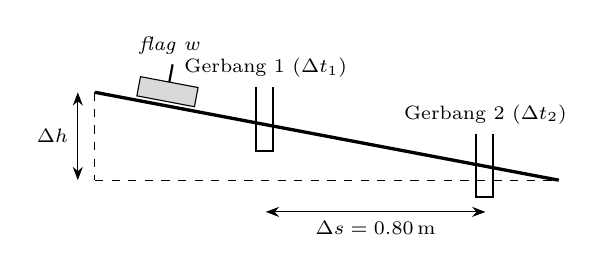
\begin{tikzpicture}[>=Stealth,scale=0.62]
  \draw[very thick] (0,2.2) -- (9.5,0.4);
  \draw[dashed] (0,0.4) -- (9.5,0.4);
  \draw[dashed] (0,2.2) -- (0,0.4);
  \draw[<->] (-0.35,0.4) -- (-0.35,2.2) node[midway,left]{\xs $\Delta h$};
  \begin{scope}[rotate=-10.7,shift={(0.45,2.2)}]
    \fill[gray!30,draw=black] (0,0.05) rectangle (1.2,0.45);
    \draw[thick] (0.60,0.45) -- (0.60,0.82);
    \node[above] at (0.55,0.82) {\xs \textit{flag} $w$};
  \end{scope}
  \draw[thick] (3.3,2.3) -- (3.3,1.0) -- (3.65,1.0) -- (3.65,2.3);
  \node[above] at (3.5,2.3) {\xs Gerbang 1 ($\Delta t_1$)};
  \draw[thick] (7.8,1.35) -- (7.8,0.05) -- (8.15,0.05) -- (8.15,1.35);
  \node[above] at (8.0,1.35) {\xs Gerbang 2 ($\Delta t_2$)};
  \draw[<->] (3.5,-0.25) -- (8.0,-0.25) node[midway,below]{\xs $\Delta s=\SI{0,80}{m}$};
\end{tikzpicture}
\capx{Gambar 1. Skema rel udara miring M3 ($g=\SI{9,806}{m/s^2}$, $\Delta h \approx \SI{28}{mm}$).}
\begin{block}{Prosedur Penapisan}\xs
Seluruh data dicatat tanpa pembulatan awal dan diuji terhadap ambang pencilan $|x_i-\bar{x}| > 3\sigma$.
\end{block}
\end{column}
\end{columns}
\end{frame}

\begin{frame}{Data Mentah P1 \& M3 ($n=8$) dan Penapisan $3\sigma$}
\begin{columns}[T,onlytextwidth]
\begin{column}{.53\textwidth}
\begin{block}{Ringkasan Data Mentah (8 Pengulangan)}\xs
\centering
\begin{tabular}{@{}ccccccc@{}}
\toprule
\textbf{Tr.} & $m$ (g) & $d$ (mm) & $h$ (mm) & $\Delta t_1$ (s) & $\Delta t_2$ (s) & $M$ (g)\\
\midrule
1 & 67,22 & 20,05 & 25,10 & 0,0521 & 0,0278 & 200,10\\
2 & 67,21 & 20,00 & 25,15 & 0,0519 & 0,0279 & 200,12\\
3 & 67,23 & 20,05 & 25,10 & 0,0523 & 0,0277 & 200,08\\
4 & 67,20 & 20,10 & 25,05 & 0,0520 & 0,0280 & 200,11\\
5 & 67,24 & 20,00 & 25,10 & 0,0522 & 0,0278 & 200,09\\
6 & 67,22 & 20,05 & 25,15 & 0,0518 & 0,0279 & 200,10\\
7 & 67,21 & 20,00 & 25,10 & 0,0524 & 0,0277 & 200,13\\
8 & 67,23 & 20,05 & 25,05 & 0,0521 & 0,0278 & 200,07\\
\bottomrule
\end{tabular}
\par\vspace{1mm}
{\xs Lebar \textit{flag} $w \approx 25{,}00\ \si{mm}$ dan $\Delta h \approx 28{,}0\ \si{mm}$.}
\end{block}
\end{column}

\begin{column}{.45\textwidth}
\begin{exampleblock}{Simpangan Maksimum ($z_{\max} = \max|x_i-\bar{x}|/s$)}\xs
\centering
\begin{tabular}{@{}lcc@{}}
\toprule
\textbf{Besaran} & $z_{\max}$ & \textbf{Status ($<3$)}\\
\midrule
Massa $m$ (P1) & 1,53 & Semua lolos\\
Diameter $d$ & 1,77 & Semua lolos\\
Tinggi $h$ & 1,32 & Semua lolos\\
Waktu $\Delta t_1$ & 1,50 & Semua lolos\\
Waktu $\Delta t_2$ & 1,69 & Semua lolos\\
Massa $M$, $w$, $\Delta h$ & 1,50 / 1,32 & Semua lolos\\
\bottomrule
\end{tabular}
\end{exampleblock}
\begin{alertblock}{Catatan Matematis Sampel Kecil}\xs
Untuk $n=8$, batas maksimum skor-$z$ sampel adalah $(n-1)/\sqrt{n} \approx 2{,}47 < 3$. Jadi $3\sigma$ secara matematis tidak dapat mendeteksi pencilan pada $n=8$; kebersihan data didukung oleh simpangan baku yang kecil.
\end{alertblock}
\end{column}
\end{columns}
\end{frame}

%=============================================================================
% SECTION 3: KARAKTERISTIK STATIS DAN DINAMIS
%=============================================================================
\section{Karakteristik Statis dan Dinamis}

\begin{frame}{Karakteristik Statis Alat Ukur (Eksperimen P1)}
\begin{columns}[T,onlytextwidth]
\begin{column}{.49\textwidth}
\begin{block}{Akurasi, Presisi, dan Repeatability}\sm
\begin{itemize}
\item \textbf{Akurasi (vs acuan $\SI{67,20}{g}$):}
  $$E_{\mathrm{abs}} = \SI{0,020}{g}, \quad E_{\mathrm{rel}} = 2{,}98\times 10^{-4}\ (0{,}030\%).$$
\item Bias $\SI{0,020}{g} > U_m = \SI{0,011}{g}$ $\implies$ signifikan secara metrologis.
\item \textbf{Presisi \& Repeatability:} $s_r = \SI{0,0131}{g}$, batas $r = 2{,}8\,s_r = \SI{0,037}{g}$.
\item \textbf{Sensitivitas OLS:} $S = 0{,}999975\ \si{g/g}$ (ideal $1{,}000000$).
\end{itemize}
\end{block}
\end{column}

\begin{column}{.49\textwidth}
\begin{exampleblock}{Uji Stabilitas: \textit{Zero Drift} Tanpa Beban}\sm
\centering
\setlength{\tabcolsep}{3.5pt}\begin{tabular}{@{}lccccccc@{}}
\toprule
\textbf{Menit} & 0 & 5 & 10 & 15 & 20 & 25 & 30\\
\midrule
\textbf{Nol (g)} & 0,00 & 0,00 & 0,01 & 0,01 & 0,02 & 0,02 & 0,03\\
\bottomrule
\end{tabular}
\par\vspace{2mm}\raggedright
\begin{itemize}
\item Pergeseran nol $+\SI{0,03}{g}$ dalam $30$ menit ($\approx \SI{1e-3}{g/menit}$), setara $3\times$ resolusi neraca.
\item Diduga akibat \textit{creep} mekanik \textit{strain gauge} dan \textit{drift} termal ADC.
\end{itemize}
\end{exampleblock}
\begin{alertblock}{Implikasi Praktis}\xs
Neraca digital wajib di-nol-kan ulang (\textit{tare}) sebelum setiap rangkaian pengukuran.
\end{alertblock}
\end{column}
\end{columns}
\end{frame}

\begin{frame}{Karakteristik Dinamis dan Efek Pembebanan (Eksperimen M3)}
\begin{columns}[T,onlytextwidth]
\begin{column}{.50\textwidth}
\begin{block}{\textit{Response Time Delay} Gerbang Cahaya ($\tau$)}\sm
Histeresis komparator menyebabkan $\Delta t_{\mathrm{ukur}} = \Delta t_{\mathrm{sejati}} - \tau$. Dengan $\tau = \SI{0,8}{ms}$ (asumsi spesifikasi):
\par\vspace{1.5mm}\centering\xs
\setlength{\tabcolsep}{3.5pt}\begin{tabular}{@{}lccc@{}}
\toprule
\textbf{Gerbang} & $v_{\mathrm{ukur}}$ (m/s) & $v_{\mathrm{terkoreksi}}$ (m/s) & \textbf{Bias (\%)}\\
\midrule
1 ($\overline{\Delta t_1} = \SI{52,10}{ms}$) & 0,4798 & 0,4726 & 1,54\\
2 ($\overline{\Delta t_2} = \SI{27,825}{ms}$) & 0,8985 & 0,8734 & 2,88\\
\bottomrule
\end{tabular}
\par\vspace{1.5mm}\raggedright\sm
Bias Gerbang~2 hampir $2\times$ lebih besar karena $\tau/\Delta t_2 > \tau/\Delta t_1$ (galat sistematis).
\end{block}
\end{column}

\begin{column}{.48\textwidth}
\begin{exampleblock}{\textit{Loading Effect} (Analogi Th\'evenin)}\sm
$$\frac{E_m}{E_o} = \frac{R_m}{R_{AB} + R_m}$$
Gesekan lapisan batas udara dan pengereman \textit{eddy current} berperan sebagai hambatan dalam mekanis $R_{AB}$ yang menyerap energi (kerangka konseptual).
\end{exampleblock}
\begin{alertblock}{\textit{Modifying Inputs} Lingkungan}\sm
\begin{itemize}
\item Embusan udara ventilasi/AC mengubah gaya hambat aerodinamis \textit{glider}.
\item Ketidakseragaman kemiringan rel mengubah nilai $\Delta h$ efektif.
\end{itemize}
\end{alertblock}
\end{column}
\end{columns}
\end{frame}

%=============================================================================
% SECTION 4: KETIDAKPASTIAN ISO-GUM
%=============================================================================
\section{Evaluasi Ketidakpastian ISO-GUM}

\begin{frame}{Evaluasi Ketidakpastian P1: Massa Jenis Kuningan ($\rho$)}
\begin{columns}[T,onlytextwidth]
\begin{column}{.49\textwidth}
\begin{block}{Formulasi ISO-GUM \& Besaran Langsung}\xs
$$\uA = \frac{s}{\sqrt{n}}, \quad \uB = \frac{\Delta x}{2\sqrt{3}}, \quad \uc = \sqrt{\uA^2+\uB^2}, \quad U = 2\uc$$
\centering
\setlength{\tabcolsep}{3.5pt}\begin{tabular}{@{}lccc@{}}
\toprule
\textbf{Parameter} & $m$ (g) & $d$ (cm) & $h$ (cm)\\
\midrule
Rata-rata $\bar{x}$ & 67,22000 & 2,00375 & 2,51000\\
$\uA$ & 0,00463 & 0,00125 & 0,00134\\
$\uB$ & 0,00289 & 0,00144 & 0,00144\\
$\uc$ & 0,00546 & 0,00191 & 0,00197\\
$U = 2\uc$ & 0,01091 & 0,00382 & 0,00393\\
\bottomrule
\end{tabular}
\end{block}
\end{column}

\begin{column}{.49\textwidth}
\begin{exampleblock}{Anggaran Ketidakpastian $\rho$}\xs
\centering
\begin{tabular}{@{}lcc@{}}
\toprule
\textbf{Sumber} & \textbf{Kontribusi $\uc(\rho)/\rho$} & \textbf{Varians (\%)}\\
\midrule
Massa $m$ & 0,00008 & 0,2\\
Diameter $d$ ($\times 2$) & 0,00191 & \textbf{85,4}\\
Tinggi $h$ & 0,00078 & 14,4\\
\midrule
\textbf{Gabungan} & \textbf{0,00206} & \textbf{100,0}\\
\bottomrule
\end{tabular}
\par\vspace{2mm}\sm
$$\boxed{\rho = (8{,}493 \pm 0{,}035)\ \si{g/cm^3}\ (k=2), \quad \frac{U}{\rho}=0{,}41\%}$$
\end{exampleblock}
\begin{alertblock}{Temuan Kunci P1}\xs
Nilai $\rho$ konsisten dengan kuningan ($\approx 8{,}4\text{--}8{,}7\ \si{g/cm^3}$). Diameter mendominasi $85{,}4\%$ varians karena resolusi jangka sorong ($\SI{0,05}{mm}$).
\end{alertblock}
\end{column}
\end{columns}
\end{frame}

\begin{frame}{Evaluasi Ketidakpastian M3: Energi Mekanik dan $\Delta E$}
\begin{columns}[T,onlytextwidth]
\begin{column}{.50\textwidth}
\begin{block}{Ketidakpastian Besaran Langsung M3}\xs
\centering
\setlength{\tabcolsep}{3.5pt}\begin{tabular}{@{}lccc@{}}
\toprule
\textbf{Besaran} & \textbf{Rata-rata} & $\uc$ & \textbf{Varians $\Delta E$ (\%)}\\
\midrule
$\Delta t_2$ (s) & 0,027825 & $4{,}66\times 10^{-5}$ & \textbf{79,6}\\
$w$ (m) & 0,025000 & $1{,}97\times 10^{-5}$ & 9,0\\
$\Delta h$ (m) & 0,028000 & $3{,}93\times 10^{-5}$ & 6,5\\
$\Delta t_1$ (s) & 0,052100 & $7{,}64\times 10^{-5}$ & 5,0\\
$M$ (kg) & 0,200100 & $7{,}64\times 10^{-6}$ & 0,0\\
\bottomrule
\end{tabular}
\par\vspace{1.5mm}\raggedright
Karena $E_1$ dan $E_2$ memakai $M$ dan $w$ yang sama, perambatan $\uc(\Delta E)$ dihitung secara berkorelasi melalui turunan parsial simbolik \texttt{SymPy}.
\end{block}
\end{column}

\begin{column}{.48\textwidth}
\begin{exampleblock}{Hasil Energi Mekanik ($k=2$)}\sm
\begin{itemize}
\item $E_{k1} = \SI{0,02304}{J}$, \quad $E_{p1} = \SI{0,05494}{J}$
\item $E_1 = (0{,}07798 \pm 0{,}00022)\ \si{J}$
\item $E_2 = (0{,}08077 \pm 0{,}00060)\ \si{J}$
\item $\boxed{\Delta E = (-2{,}79 \pm 0{,}61)\times 10^{-3}\ \si{J}}$
\end{itemize}
{\xs (Tanpa korelasi memberi $U(\Delta E)=\SI{0,00064}{J}$, kesimpulan tetap sama.)}
\end{exampleblock}
\begin{alertblock}{Anomali Fisis $\Delta E < 0$}\xs
Selisih $\Delta E$ bernilai negatif sekitar $4{,}6\,U$ dari nol, seolah energi bertambah; ini menandakan adanya galat sistematis yang lebih besar dari $U(\Delta E)$.
\end{alertblock}
\end{column}
\end{columns}
\end{frame}

%=============================================================================
% SECTION 5: KALIBRASI DAN VALIDASI
%=============================================================================
\section{Kalibrasi OLS dan Analisis Residual}

\begin{frame}{Kalibrasi Neraca Digital dan Uji Linearitas}
\begin{columns}[T,onlytextwidth]
\begin{column}{.48\textwidth}
\begin{block}{Data Kalibrasi 8 Titik (Kelas F2)}\xs
\centering
\begin{tabular}{@{}cccc@{}}
\toprule
$x$ \textbf{std (g)} & $y$ \textbf{baca (g)} & $\hat{y}$ \textbf{(g)} & \textbf{Residual $e_i$ (g)}\\
\midrule
10,00 & 10,02 & 10,0419 & $-0{,}0219$\\
20,00 & 20,03 & 20,0416 & $-0{,}0116$\\
50,00 & 50,04 & 50,0409 & $-0{,}0009$\\
100,00 & 100,06 & 100,0396 & $+0{,}0204$\\
150,00 & 150,07 & 150,0384 & $+0{,}0316$\\
200,00 & 200,05 & 200,0371 & $+0{,}0129$\\
250,00 & 250,03 & 250,0359 & $-0{,}0059$\\
300,00 & 300,01 & 300,0346 & $-0{,}0246$\\
\bottomrule
\end{tabular}
\end{block}
\end{column}

\begin{column}{.50\textwidth}
\begin{exampleblock}{Parameter Regresi OLS}\sm
$$\boxed{y = 0{,}999975\,x + 0{,}0421\ \si{g}, \quad R^2 = 0{,}99999997}$$
\begin{itemize}
\item $s_{y/x} = \SI{0,0217}{g}$, $u(a)=7{,}6\times 10^{-5}$, $u(b)=\SI{0,013}{g}$.
\item $|a-1| < u(a)$ $\implies$ sensitivitas tidak berbeda nyata dari ideal.
\item Intersep $b = \SI{0,042}{g}$ ($\approx 3{,}3\,u(b)$) sejalan dengan \textit{zero drift} ($\SI{0,03}{g}$).
\end{itemize}
\end{exampleblock}
\begin{alertblock}{Jebakan $R^2 \approx 1$}\xs
Regresi kuadratik menurunkan $s_{y/x}$ menjadi $\SI{0,0056}{g}$ ($c_2 = -2{,}3\times 10^{-6}\ \si{g^{-1}}$). Meskipun $R^2 \approx 1$, residual berpola busur terbalik hingga $\SI{0,032}{g}$.
\end{alertblock}
\end{column}
\end{columns}
\end{frame}

\begin{frame}{Visualisasi Kurva Kalibrasi, Residual, dan 5 Uji Validasi}
\begin{columns}[T,onlytextwidth]
\begin{column}{.56\textwidth}
\centering
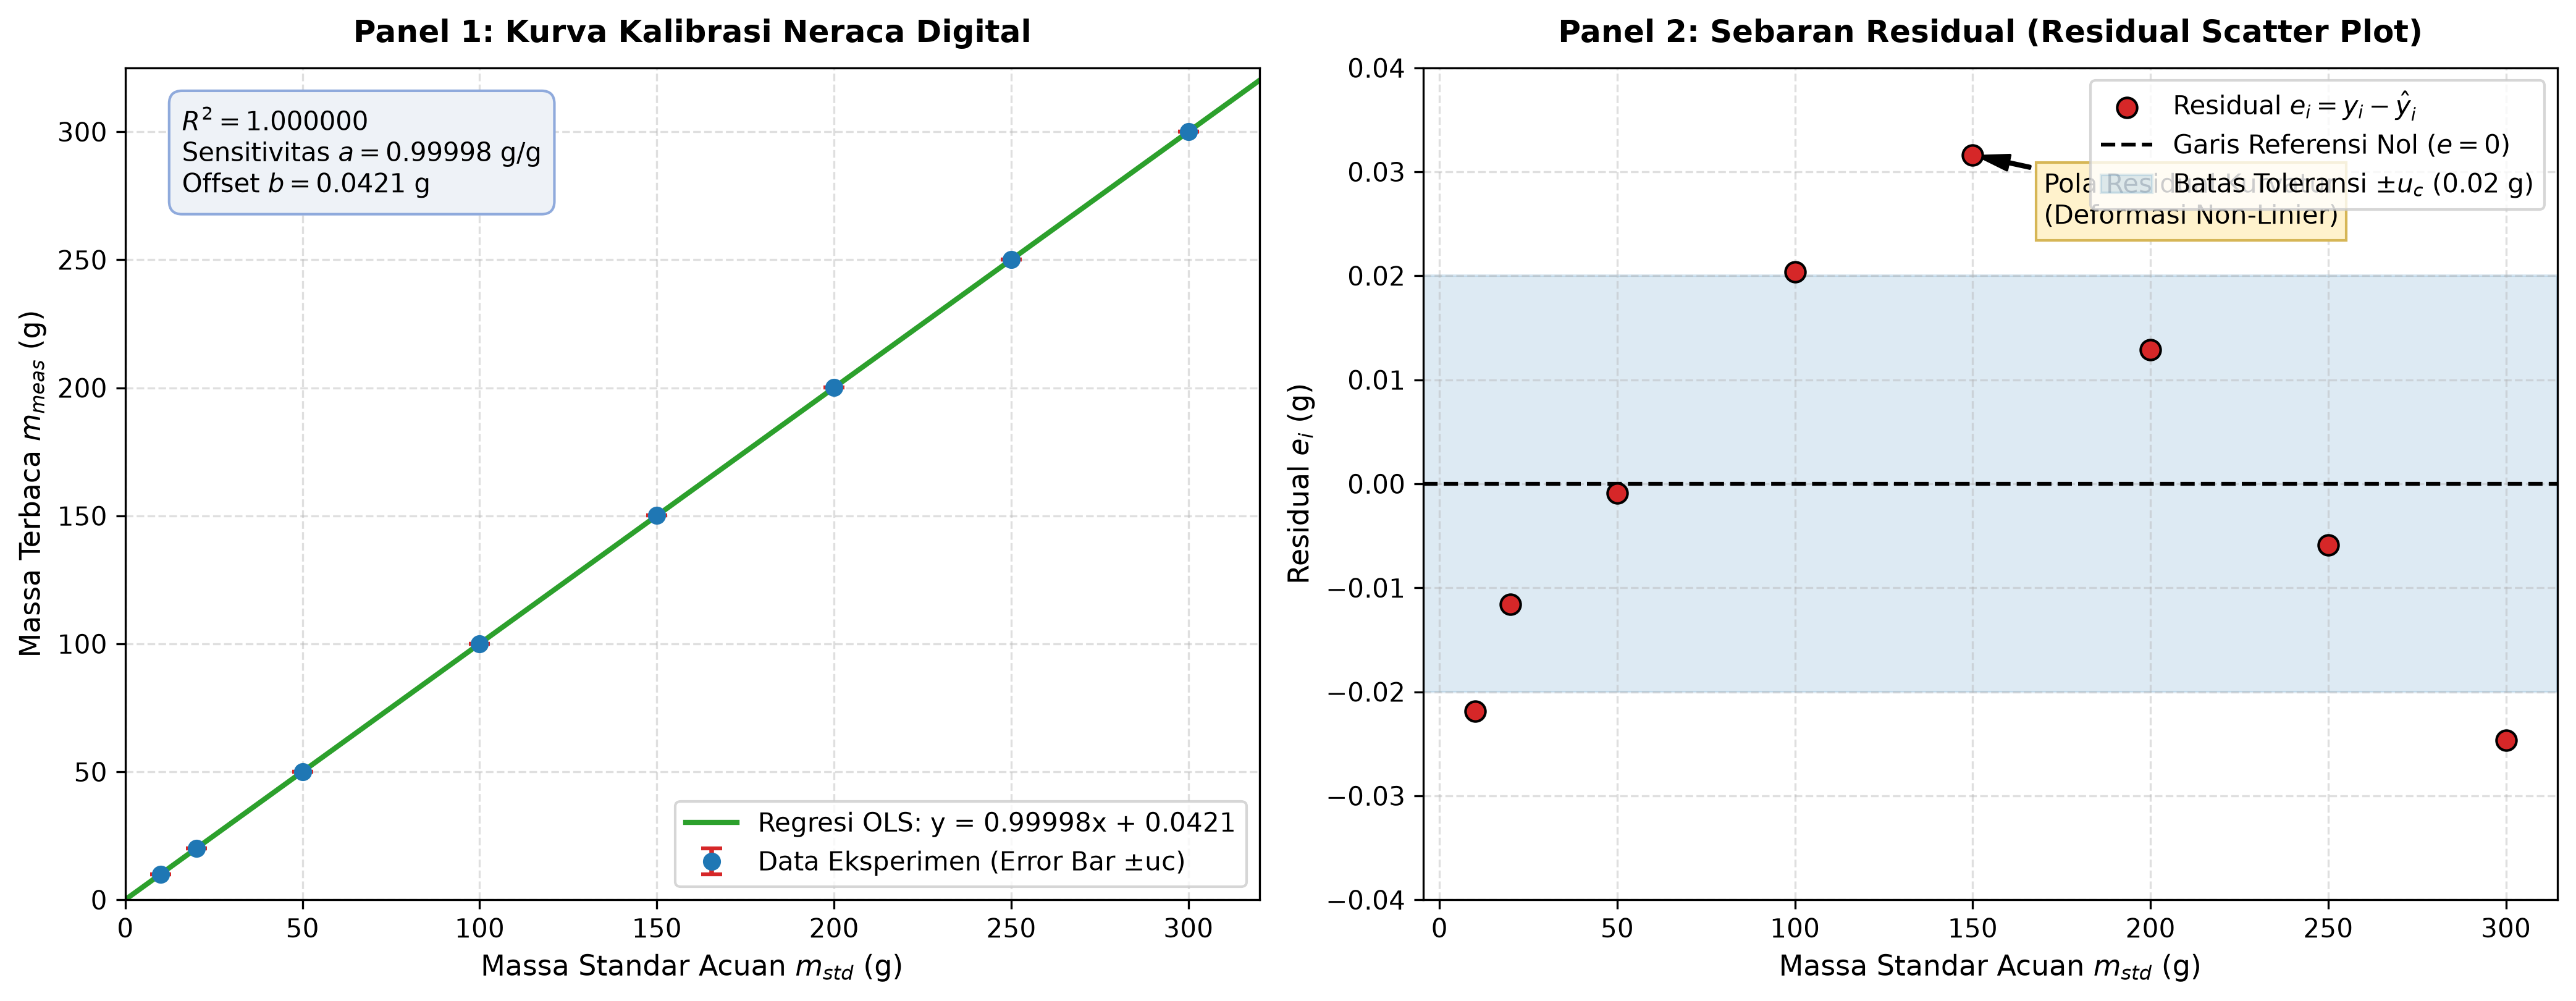
\includegraphics[width=\linewidth,keepaspectratio]{Images/Kalibrasi_Residual.png}
\capx{Gambar 2. Kurva kalibrasi OLS (kiri) dan pola residual non-acak berpola lengkung (kanan).}
\end{column}

\begin{column}{.42\textwidth}
\begin{block}{Ringkasan 5 Uji Validasi}\xs
\begin{enumerate}
\item \textbf{Accuracy:} Bias P1 $\SI{0,020}{g}$ ($> U_m$); galat kalibrasi maks. $+\SI{0,07}{g}$ pada $\SI{150}{g}$.
\item \textbf{Repeatability:} $s_r=\SI{0,0131}{g}$, $r=\SI{0,037}{g}$ ($\approx 1$ digit).
\item \textbf{Linearity:} Simpangan maks. $\SI{0,032}{g}$ ($0{,}011\%$ FS), pola lengkung.
\item \textbf{Functional:} Stabil pada $2$ desimal, perlu \textit{zeroing} berkala.
\item \textbf{Response/Stability:} \textit{Zero drift} $+\SI{0,03}{g}/30$ mnt; tunda gerbang cahaya $\approx \SI{0,8}{ms}$.
\end{enumerate}
\end{block}
\end{column}
\end{columns}
\end{frame}

%=============================================================================
% SECTION 6: DISKUSI, KESIMPULAN, DAN REFERENSI
%=============================================================================
\section{Diskusi, Kesimpulan, dan Referensi}

\begin{frame}{Analisis Reflektif ``So What?'': Diagnosis Galat Sistematis}
\begin{columns}[T,onlytextwidth]
\begin{column}{.48\textwidth}
\begin{block}{Eksperimen P1 (Statis)}\sm
\begin{itemize}
\item $\rho = (8{,}493 \pm 0{,}035)\ \si{g/cm^3}$ mengidentifikasi bahan sebagai kuningan, namun $0{,}41\%$ belum membedakan rasio Cu--Zn.
\item Mengganti jangka sorong ($\SI{0,05}{mm}$) dengan mikrometer ($\SI{0,01}{mm}$) untuk $d$ menurunkan $U(\rho)$ menjadi $\sim \SI{0,026}{g/cm^3}$ (jauh lebih efektif daripada menambah ulangan massa).
\end{itemize}
\end{block}
\begin{exampleblock}{Komparasi Statis vs Dinamis}\xs
Galat statis (P1) didominasi acak/resolusi, sedangkan galat dinamis (M3) didominasi tunda $\tau$ yang lolos uji $3\sigma$.
\end{exampleblock}
\end{column}

\begin{column}{.50\textwidth}
\begin{alertblock}{Eksperimen M3: Mengapa $\Delta E < 0$?}\sm
\begin{enumerate}
\item \textbf{Response time delay ($\tau$):} Karena $v_2$ ter-\textit{overestimate} lebih besar daripada $v_1$, koreksi $\tau=\SI{0,8}{ms}$ membalik hasil menjadi $\Delta E = +\SI{0,97e-3}{J}$ (disipasi positif wajar). Titik nol $\Delta E = 0$ terjadi pada $\tau \approx \SI{0,59}{ms}$.
\item \textbf{Ketidakakuratan $\Delta h$:} Memerlukan $\Delta h \approx \SI{29,4}{mm}$ ($+1{,}4\ \si{mm} \approx 18\,U(\Delta h)$), kecil peluang sebagai penyebab tunggal.
\item \textbf{Kecepatan sesaat vs rata-rata:} $v=w/\Delta t$ mengukur rata-rata selama interupsi \textit{flag}.
\end{enumerate}
\end{alertblock}
\end{column}
\end{columns}
\end{frame}

\begin{frame}{Kesimpulan dan Rekomendasi Teknis}
\begin{columns}[T,onlytextwidth]
\begin{column}{.49\textwidth}
\begin{block}{Kesimpulan Utama}\sm
\begin{enumerate}
\item Massa jenis kuningan $\rho = (8{,}493 \pm 0{,}035)\ \si{g/cm^3}$ ($k=2$); diameter menyumbang $85{,}4\%$ varians.
\item Kalibrasi OLS $y = 0{,}999975\,x + 0{,}0421$ ($R^2 \approx 1$) menyembunyikan pola residual lengkung ($\max \SI{0,032}{g}$).
\item $\Delta E = (-2{,}79 \pm 0{,}61)\times 10^{-3}\ \si{J}$ disebabkan oleh galat sistematis dinamis ($\tau$ gerbang cahaya), bukan pelanggaran kekekalan energi.
\end{enumerate}
\end{block}
\end{column}

\begin{column}{.49\textwidth}
\begin{exampleblock}{Rekomendasi Teknis Laboratorium}\sm
\begin{enumerate}
\item \textbf{Ukur $\tau$ gerbang cahaya} dengan osiloskop dan terapkan $\Delta t_{\mathrm{sejati}} = \Delta t_{\mathrm{ukur}} + \tau$.
\item \textbf{Gunakan mikrometer sekrup} untuk $d$ dan $h$ pada P1.
\item \textbf{Verifikasi kemiringan rel} (\textit{spirit level}) dan ukur $\Delta h$ lebih halus dari $\SI{0,1}{mm}$.
\item \textbf{Lakukan \textit{tare} berkala}, tambah titik kalibrasi ($50\text{--}200\ \si{g}$), dan pasang \textit{draft shield} akrilik.
\end{enumerate}
\end{exampleblock}
\end{column}
\end{columns}
\end{frame}

\begin{frame}{Daftar Pustaka}
\xs
\begin{enumerate}
\item Bentley, J. P. (2005). \emph{Principles of Measurement Systems} (4th ed.). Pearson Education.
\item Halliday, D., Resnick, R., \& Walker, J. (2013). \emph{Fundamentals of Physics}. John Wiley \& Sons.
\item Joint Committee for Guides in Metrology. (2008). \emph{Evaluation of Measurement Data --- Guide to the Expression of Uncertainty in Measurement (GUM)}, JCGM 100:2008. BIPM.
\item Joint Committee for Guides in Metrology. (2012). \emph{International Vocabulary of Metrology --- Basic and General Concepts and Associated Terms (VIM)}, JCGM 200:2012. BIPM.
\item Morris, A. S., \& Langari, R. (2012). \emph{Measurement and Instrumentation: Theory and Application}. Academic Press.
\item Taylor, J. R. (1997). \emph{An Introduction to Error Analysis: The Study of Uncertainties in Physical Measurements} (2nd ed.). University Science Books.
\item Yhuwana, Y. G. Y. (2026). \emph{Modul Panduan Praktikum dan Lembar Kerja Mahasiswa (LKM): Case-Based Learning dan Elaborative Project Pengukuran Fisika}. FIT310 Sensor dan Pengukuran, Program Studi Fisika, Universitas Airlangga.
\end{enumerate}
\vspace{2mm}
\begin{exampleblock}{Reprodusibilitas Komputasi}\xs
Seluruh kalkulasi simbolik (\texttt{SymPy}), regresi OLS, grafik, dan ekspor Excel tersedia pada \texttt{Instrumentation\_Calibration\_Analysis.ipynb} dan \texttt{Instrumentation\_Calibration\_Data.xlsx}.
\end{exampleblock}
\end{frame}

%=============================================================================
% CLOSING SLIDE
%=============================================================================
\begin{frame}[plain]
\centering
\vfill

\includegraphics[height=2.2cm,keepaspectratio]{Images/logo-unair.png}
\vspace{4mm}

{\color{navy}\Huge\bfseries TERIMA KASIH\par}
\vspace{2mm}
{\Large Sesi Diskusi dan Tanya Jawab\par}
\vspace{4mm}

\parbox{0.74\linewidth}{%
  \begin{beamercolorbox}[wd=\linewidth,sep=7pt,center,rounded=true]{block body}
    \centering\sm
    Program Studi Fisika, Departemen Fisika\par\vspace{1mm}
    Fakultas Sains dan Teknologi\par\vspace{1mm}
    Universitas Airlangga --- 2026
  \end{beamercolorbox}%
}

\vfill
\end{frame}

\end{document}
